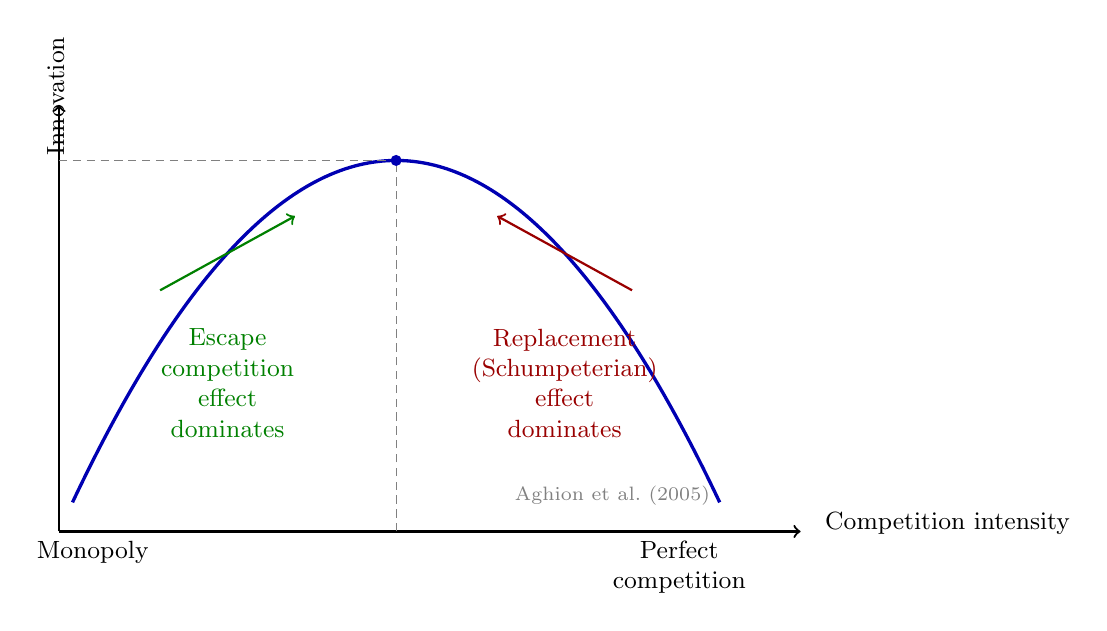
\begin{tikzpicture}
\begin{axis}[
  width=11cm, height=7cm,
  xmin=0, xmax=1.1,
  ymin=0, ymax=1.15,
  axis lines=left,
  axis line style={thick, ->},
  ticks=none,
  clip=false,
  xlabel={Competition intensity},
  ylabel={Innovation},
  xlabel style={at={(axis description cs:1.02,0.02)}, anchor=west, font=\small},
  ylabel style={at={(axis description cs:0.02,1.02)}, anchor=south, font=\small},
]

% Inverted-U curve: y = 4x(1-x) scaled
\addplot[very thick, domain=0.02:0.98, samples=200, color=blue!70!black]
  {4*x*(1-x)};

% Peak
\pgfmathsetmacro{\xpeak}{0.5}
\pgfmathsetmacro{\ypeak}{1.0}

% Dashed lines to peak
\addplot[densely dashed, thin, gray] coordinates {(\xpeak,0) (\xpeak,\ypeak)};
\addplot[densely dashed, thin, gray] coordinates {(0,\ypeak) (\xpeak,\ypeak)};

% Peak dot
\fill[blue!70!black] (axis cs:\xpeak,\ypeak) circle (2pt);

% Region labels
\node[font=\small, align=center, text=green!50!black] at (axis cs:0.25,0.4)
  {Escape\\competition\\effect\\dominates};

\node[font=\small, align=center, text=red!60!black] at (axis cs:0.75,0.4)
  {Replacement\\(Schumpeterian)\\effect\\dominates};

% Arrow annotations
\draw[->, thick, green!50!black] (axis cs:0.15,0.65) -- (axis cs:0.35,0.85);
\draw[->, thick, red!60!black] (axis cs:0.85,0.65) -- (axis cs:0.65,0.85);

% X-axis labels
\node[anchor=north, font=\small] at (axis cs:0.05,0) {Monopoly};
\node[anchor=north, font=\small, align=center] at (axis cs:0.92,0) {Perfect\\competition};

% Source annotation
\node[anchor=north east, font=\scriptsize, gray] at (axis cs:0.98,0.15)
  {Aghion et al.\ (2005)};

\end{axis}
\end{tikzpicture}
